%%% License: Creative Commons Attribution Share Alike 4.0 (see https://creativecommons.org/licenses/by-sa/4.0/)

\documentclass[english,10pt
,aspectratio=169
%,handout
%,notes
]{beamer}
%%% License: Creative Commons Attribution Share Alike 4.0 (see https://creativecommons.org/licenses/by-sa/4.0/)

\DeclareGraphicsExtensions{.eps, .pdf,.png,.jpg,.mps,}
\usetheme{reMedian}
\usepackage{parskip}
\makeatother

\renewcommand{\baselinestretch}{1.1} 

\usepackage{amsmath, amssymb, amsfonts, amsthm}
\usepackage{enumerate}
%\usepackage{enumitem}
\usepackage{hyperref}
\usepackage{url}
\usepackage{bbm}
\usepackage{color}

\usepackage{tikz}
\usepackage{tikzscale}
\newcommand*\circled[1]{\tikz[baseline=(char.base)]{
		\node[shape=circle,draw, inner sep=-20pt] (char) {#1};}}
\usetikzlibrary{automata,positioning}
\usetikzlibrary{decorations.pathreplacing}
\usepackage{pgfplots}
\usepgfplotslibrary{fillbetween}
\usepackage{graphicx}

\usepackage{setspace}
\thinmuskip=1mu
\medmuskip=1mu 
\thickmuskip=1mu 


\usecolortheme{default}
\usepackage{verbatim}
\usepackage[normalem]{ulem}

\usepackage{apptools}
\AtAppendix{
	\setbeamertemplate{frame numbering}[none]
}
\usepackage{natbib}


% red strikeout
\newcommand\soutred{\bgroup\markoverwith
	{\textcolor{red}{\rule[0.55ex]{2pt}{0.8pt}}}\ULon}



% To use LyX frames from old version:
\def\lyxframeend{} % In case there is a superfluous frame end
\long\def\lyxframe#1{\@lyxframe#1\@lyxframestop}%
\def\@lyxframe{\@ifnextchar<{\@@lyxframe}{\@@lyxframe<*>}}%
\def\@@lyxframe<#1>{\@ifnextchar[{\@@@lyxframe<#1>}{\@@@lyxframe<#1>[]}}
\def\@@@lyxframe<#1>[{\@ifnextchar<{\@@@@@lyxframe<#1>[}{\@@@@lyxframe<#1>[<*>][}}
\def\@@@@@lyxframe<#1>[#2]{\@ifnextchar[{\@@@@lyxframe<#1>[#2]}{\@@@@lyxframe<#1>[#2][]}}
\long\def\@@@@lyxframe<#1>[#2][#3]#4\@lyxframestop#5\lyxframeend{%
	\frame<#1>[#2][#3]{\frametitle{#4}#5}}


\title{Mechanism Design}

\subtitle{4: Correlated Information}

\author{Egor Starkov}

\date{K{\o}benhavns Unversitet \\
	Fall 2020}


\begin{document}
	\AtBeginSection[]{
		\frame{
			\frametitle{This slide deck:}
			\tableofcontents[currentsection,currentsubsection]
	}}
	\frame[plain]{\titlepage}



\begin{frame}{Independent vs Correlated Information}
\begin{itemize}
	\item So far we always assumed types $\theta_i$ \structure{independently} distributed.
	\begin{itemize}
		\item Not an innocuous assumption.
		\item Very important for results (esp. BIC mechanisms -- DSIC are not affected because DS).
	\end{itemize}
	\item What if types are \alert{correlated}? Does it hurt or help?
	\begin{itemize}
		\item If $\theta_i$ are correlated then each $i$ has some information about all $\theta_j$.
		\item Can use it to cross-check reports of $\theta_j$.
	\end{itemize}
\end{itemize}
\end{frame}


\section{Perfect correlation}

\begin{frame}{Perfect Correlation}
\begin{itemize}
	\item Consider a \structure{quasilinear} setting with modification.
	\item $N$ agents with \structure{perfectly correlated} types: $\theta_i = \omega$ $\forall i$.
	\item Designer does not know $\omega \in \Omega$, only knows the distribution $F(\omega)$ (as usual).
	\item Designer wants to implement some allocation $k(\omega)$.
\end{itemize}
\end{frame}
\note{
	Recall that types have dual role as describing
	\begin{itemize}
		\item own preferences
		\item info about others' preferences.
	\end{itemize}
	If we interpret this as trade setting, with types as valuations: differences between this problem and uncorr types is in info about others' prefs, but not in own prefs.
}


\begin{frame}{Perfect Correlation}
\begin{itemize}
	\item Consider the following direct mechanism:
	\begin{itemize}
		\item \structure{If} all agents' reports \structure{agree} ($\hat{\theta}_i=\hat{\theta}_j=\hat{\omega}$ for all $i,j$) then implement $k(\hat{\omega})$ with zero transfers.
		\item \alert{Otherwise} implement any $k \in K$ and set \alert{$t_i = +\infty$} for all $i$.
		\item (If the desired s.c.f. $k(\theta)$ prescribes an allocation to mismatching types, can use that instead.)
	\end{itemize}
	\item This mechanism truthfully implements $k(\omega)$ (BIC? DSIC?).
	\begin{itemize}
		\item Never profitable to deviate alone (then must pay infinity).
		\item There are also many other equilibria apart from truthful one...
		\item[Q:] In truthful eqm, would $t_i = +\infty$ after disagreement interfere with IR? (if we care about IR)
	\end{itemize}
\end{itemize}
\end{frame}


\section{Imperfect correlation}

\begin{frame}{Imperfect correlation: setup}
\begin{itemize}
	\item Still a \structure{quasilinear world} with modification.
	\item $N$ agents with private types $\theta_i \in \Theta_i$ ($\Theta_i$ finite).
	\item Types have some joint distribution: $(\theta_1,...,\theta_N) \sim \phi(\Theta)$.
	\item Player $i$'s beliefs about $\theta_{-i}$ are derived by Bayes' rule:
	$$\phi(\theta_{-i}|\theta_i) = \frac{\phi(\theta_{-i},\theta_i)}{\sum_{\theta_{-i}' \in \Theta_{-i}} \phi(\theta_{-i}',\theta_i)} $$
	\item Designer only knows the distribution $F$, wants to implement some allocation $k(\theta)$.
\end{itemize}
\end{frame}


\begin{frame}{Imperfect correlation: a simple example}
\begin{example}[2x2]
	\begin{center}
		\begin{tabular}{c | c | c |}
			 & H 				& L					\\ \hline
			H	& $\frac{1}{6}$ 	& $\frac{1}{3}$ 	\\ \hline
			L	& $\frac{1}{3}$ 	& $\frac{1}{6}$		\\ \hline
		\end{tabular}
	\end{center}
	\begin{itemize}
		\item 2 agents, 2 types each: $\theta_i \in \{H,L\}$, joint distribution $\phi(\theta_1,\theta_2)$ in the table above.
		\item Each agent thinks $\theta_j = \theta_i$ is twice less likely than otherwise. 
	\end{itemize}
\end{example}
\end{frame}


\begin{frame}{Imperfect correlation}
\begin{itemize}
	\item A similar idea can be used as with perfect correlation.
	\item Now $i$ does not know $\theta_j$ perfectly -- can't use this info to cross-verify.
	\item But can force $i$ to gamble on $\theta_j$.
	%\item Forget about the allocation rule $k$. Focus on gambles over other's types.
\end{itemize}
\end{frame}


\begin{frame}{Cremer-McLean condition}
\begin{itemize}
	\item Write your beliefs $\phi(\theta_{-i}|\theta_i)$ as a vector $\tilde\phi(\theta_i)$ (for each $\theta_{-i}\in\Theta_{-i}$ one entry in the vector).
	\item Cremer-McLean condition: no such vector $\tilde\phi(\theta_i)$ is a linear combination of the other vectors in $\{\tilde\phi(\theta_i'):\;\theta_i\neq\theta_i'\in\Theta_i\}$
\end{itemize}

\begin{definition}[CM condition]
	The distribution $\phi$ satisfies the \structure{CM condition} if there are no agent $i$ with type $\theta_i\in\Theta_i$ and weights $\lambda_i: \Theta_i\setminus\{\theta_i\} \to \mathbb{R}_+$ such that
	\begin{equation*}
		\phi(\theta _{-i}|\theta _i)=\sum_{\theta _i'\in\Theta_i\setminus\{\theta_i\}}\lambda_i(\theta_i')\phi(\theta_{-i}|\theta_i')\qquad\text{for all }\theta_{-i}\in\Theta_{-i}.
	\end{equation*}
\end{definition}
\end{frame}


\begin{frame}{Cremer-McLean condition}
\begin{itemize}
	\item Stack vectors $\tilde\phi(\theta_i)$ for each type $\theta_i$ into a matrix.
	\item The condition holds if this matrix has full rank.
	\item In particular, every type $\theta_i$ must have its own distinct belief about the distribution of $\theta_{-i}$ (but the condition is stronger than this).
	\item Does the condition hold in the 2x2 example?
	\item How about in the following:
	\begin{example}[2x3]
		\begin{center}
			\begin{tabular}{c | c | c | c |}
					& H 				& M				& L					\\ \hline
				H	& $\frac{1}{12}$ 	& $\frac{1}{4}$ & $\frac{1}{6}$ 	\\ \hline
				L	& $\frac{1}{6}$ 	& $\frac{1}{4}$ & $\frac{1}{12}$		\\ \hline
			\end{tabular}
		\end{center}
	\end{example}
\end{itemize}
\end{frame}


\begin{frame}{Cremer-McLean result}
\begin{theorem}[Cremer-McLean]
	If $\phi$ satisfies the CM condition, then for any mechanism $(k,t)$ there is a direct mechanism $(k,t')$ such that
	\begin{itemize}
		\item $(k,t')$ is \alert{BIC},
		\item both mechanisms have the same allocation $k$,
		\item both mechanisms have the same interim expected payoffs: $\forall i,\theta_i$,
	\end{itemize}
	\begin{equation*}
		%\sum_{\theta _{-i}\in\Theta _{-i}}t_i(\theta _i,\theta _{-i})\phi(\theta _{-i}|\theta _i)=  \sum_{\theta _{-i}\in\Theta _{-i}}t_i'(\theta _i,\theta _{-i})\phi(\theta _{-i}|\theta _i)
		\mathbb{E}_{\theta_{-i}} \left[ t_i(\theta) | \theta_i \right] = \mathbb{E}_{\theta_{-i}} \left[ t_i'(\theta) | \theta_i \right]
	\end{equation*}
\end{theorem}
\begin{itemize}
	\item Holds for \structure{any} mechanism $(k,t)$ -- IC not required!
	\item Meaning \structure{any} allocation rule \structure{$k$ is BIC} if $\phi$ satisfies CM condition!
\end{itemize}
\end{frame}


\begin{frame}{Proof Idea}
Forget about the allocation \(k\) and think about how to elicit private information truthfully.
\begin{example}[Information elicitation]
	\begin{itemize}
		\item State of the world $\omega \in \Omega$; expert knows true distribution $\pi$ of states (but not the state); designer knows nothing.
		\item How to extract information about $\pi$ from the expert?
		\item Consider the following scheme:
		\begin{itemize}
			\item the expert announces a probability distribution $\hat{\pi}$;
			\item when state $\omega$ realizes, the expert is paid $\log(\hat{\pi}(\omega))$
		\end{itemize}
		{\footnotesize
			\begin{align*}
				\text{Expert's problem: } & \max_{\hat{\pi}}\sum_{\omega\in\Omega} \pi(\omega) log(\hat{\pi}(\omega))
				\\
				&\text{subject to } \sum_{\omega\in\Omega} \hat{\pi}(\omega)=1.
			\end{align*}
			\vspace{-1ex}
		}
		\item Solve using Lagrange method to see that truthful reporting is optimal.
	\end{itemize}
\end{example}
\end{frame}


\begin{frame}{Proof Idea}
	\begin{block}{Proof idea}
		\begin{itemize}
			\item In our mechanism design problem, consider transfers
			$$t'_i(\theta_i,\theta_{-i}) = t_i(\theta_i,\theta_{-i}) + C_{i,1} - C_{i,2} \log (\phi(\theta_{-i}|\theta_i)).$$
			\item If $C_{i,2}$ is large enough, $i$'s incentives are dominated by the need to report $\phi(\theta_{-i}|\theta_i)$ correctly (rather than desire to get best $k(\theta)$).
			\item So set $C_{i,2}$ large, then use $C_{i,1}$ to adjust the averages as required and voila. ``$\square $''
		\end{itemize}
	\end{block}
\begin{itemize}
	\item The above is \alert{not a complete proof}, since we would actually want $C_{i,1}$ to depend on $\theta_i$ to get $\mathbb{E}_{\theta_{-i}} \left[ t_i(\theta) | \theta_i \right] = \mathbb{E}_{\theta_{-i}} \left[ t_i'(\theta) | \theta_i \right]$ $\forall i,\theta_i$. Otherwise we only have $\mathbb{E}_{\theta} \left[ t_i(\theta) \right] = \mathbb{E}_{\theta} \left[ t_i'(\theta) \right]$ $\forall i$.
	\begin{itemize}
		\item But making $C_{i,1}(\theta_i)$ depend on $\theta_i$ affects reporting incentives...
	\end{itemize}
	\item For full proof (and construction) see B{\"o}rgers ch6.4 or \href{https://www.jstor.org/stable/1913096}{\uline{Cremer \& McLean (1988)}}.
\end{itemize}
\end{frame}


\begin{frame}{Conclusion}
\begin{itemize}
	\item Cremer-McLean result is a VERY powerful tool to implement literally anything under correlated information.
	\item \textbf{Issues:}
	\item Strong-ish condition on $\phi$ --
	\begin{itemize}
		\item this method cannot extract private information which does not affect $i$'s belief about $\theta_{-i}$.
		\item But we can use it as a first step to extract some info, then proceed as before.
	\end{itemize}
	\item With weak correlation $C_{i,2}$ can be HUGE,
	\begin{itemize}
		\item leading to extremely large (positive and negative) $t_i(\theta)$.
		\item Not good if want \emph{ex post} IR, \emph{ex post} BB, and/or \emph{limited liability} ($t_i(\theta)\leq 0$ -- reasonable requirement in some settings, close to ex post IR).
	\end{itemize}
\end{itemize}
\end{frame}


\section{Perfect correlation, no commitment}

\begin{frame}{Setup}
\begin{itemize}
	\item Example based on \href{https://onlinelibrary.wiley.com/doi/abs/10.1111/1468-0262.00336}{\uline{Battaglini (2003)}}.
	\item Two \structure{agents}, $i \in \{1,2\}$:
	\begin{itemize}
		\item \emph{both} know \alert{state} $\omega = (\omega^1,\omega^2) \in \mathbb{R}^2$;
		\item each sends \alert{report} $m \in \mathbb{R}^2$ to the principal.
	\end{itemize}
	\item \structure{Principal} (``designer'') does not know $\omega$, must choose action $a \in \mathbb{R}^2$ after hearing $(m_1,m_2)$.
	\item Preferences: squared Euclidean distance between $a$ and resp. \alert{bliss points}
	\begin{itemize}
		\item Principal: $u_p (a,\omega) = -\left(\left\|a-\omega\right\| \right)^2$;
		\item Agent $i$: $u_i (a,\omega) = -\left(\left\|a-(\omega+b_i)\right\| \right)^2$;
		\item where $\left\|x\right\| \equiv \sqrt{(x^1)^2 + (x^2)^2}$ for $x = (x^1,x^2) \in \mathbb{R}^2$.
		\item \alert{Biases} $b_i$ commonly known.
	\end{itemize}
	\item (Subscripts index $i$, superscripts stand for coordinates [in default basis] and exponents.)
\end{itemize}
\end{frame}


\begin{frame}{Motivation}
\begin{itemize}
	\item You can see this as a ``level-1'' mechanism design problem in our classification:
	{\footnotesize 
	\begin{description}
		\item[Level 1:] \structure{check whether some given s.c.f $x(\theta)$ is implementable.}
		\item[Level 2:] design transfers $t(\theta)$ to implement some $k(\theta)$.
		\item[Level 3:] design $(k(\theta),t(\theta))$ or $x(\theta)$ to maximize some objective function.
	\end{description}
	}
	%\item Not a ``mechanism design problem''...
	%\begin{itemize}
	%	\item \alert{no commitment} for principal -- cannot really ``design'' any \structure{incentive structure} for agents.
	%\end{itemize}
	%\item ...but can ask a related question: how to design \structure{communication}?
	%\begin{itemize}
	%	\item Choose what information should be contained in agents' reports.
	%\end{itemize}
	\item ...where the objective is $a(\omega) = \omega$ (\structure{perfect revelation} of information).
	\item However, this is not quite a MD problem because the principal \alert{cannot commit} to a mechanism,
	\begin{itemize}
		\item since action $a(m_1,m_2)$ must maximize $u_p$, principal cannot commit to other actions (e.g. threaten with $a=(\infty,\infty)$ if agents' reports disagree),
		\item so we cannot use the revelation principle. So the question is:
		\begin{block}{}
			\alert{What} should agents be asked to report, for truthtelling to be an equilibrium?
		\end{block}
	\end{itemize}
\end{itemize}
\end{frame}


\begin{frame}{Remark: a view from a different angle}
\begin{itemize}
	%\item Why is this a meaningful question given lack of commitment?
	\item Games of \structure{communication} via ``cheap talk'' have \alert{\textbf{many} equilibria}. 
	\begin{itemize}
		\item Main reason: it takes two to talk, so a single player cannot deviate to more informative communication.
		\item Even if both sender and receiver could benefit from informative communication, they can be trapped in uninformative equilibrium.
		\item If I say gibberish and you ignore everything I say, this is \emph{always} an equilibrium, regardless of the underlying game. (See next slide for an illustration from the animal kingdom.)
		%\item (You can't hear anything valuable if you try; I can't convey anything meaningful because you won't listen.)
		\item The same applies to ``slightly informative equilibrium''... and ``moderately informative equilibrium''...
		\item And there can be many ``slightly informative equilibria'' that have different kinds of noise in messages... You see now where the multiplicity comes from?
	\end{itemize}
	\item Our ``\structure{Communication Design}'' problem is effectively an \structure{equilibrium selection} issue: does there exist a communication norm (language, possibly established by principal), under which all information is revealed in our model?
\end{itemize}
\end{frame}


\begin{frame}
	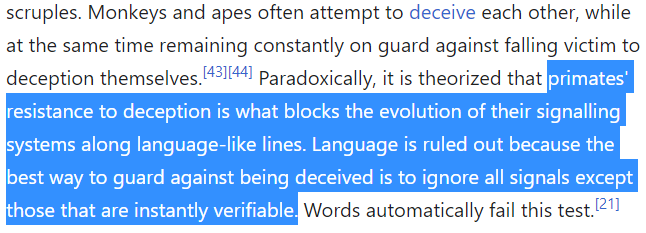
\includegraphics[scale=1.05]{pics/M4/cheaptalkmonke.png}
	\medskip
	
	\url{https://en.wikipedia.org/wiki/Origin_of_language\#Problems_of_reliability_and_deception}
\end{frame}


\begin{frame}{Idea}
\begin{columns}
	\begin{column}{0.5\textwidth}
		\begin{center}
			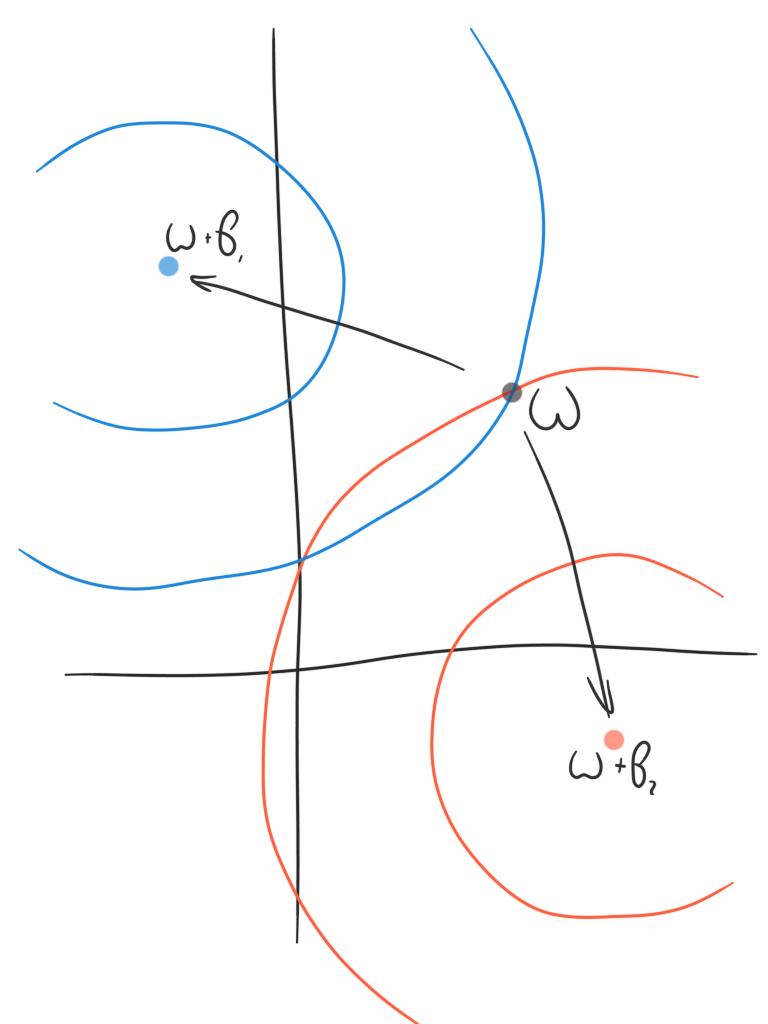
\includegraphics[scale=0.65]{pics/M4/battaglini01.png}
		\end{center}
	\end{column}
	\begin{column}{0.5\textwidth}
		{\small
			\begin{itemize}
				\item Relative positions of bliss points and indifference curves are fixed; just the absolute location unknown.
				\item The circles on the graph represent the indifference curves of the two players.
			\end{itemize}
		}
	\end{column}
\end{columns}
\end{frame}


\begin{frame}{Idea}
\begin{columns}
	\begin{column}{0.5\textwidth}
		\begin{center}
			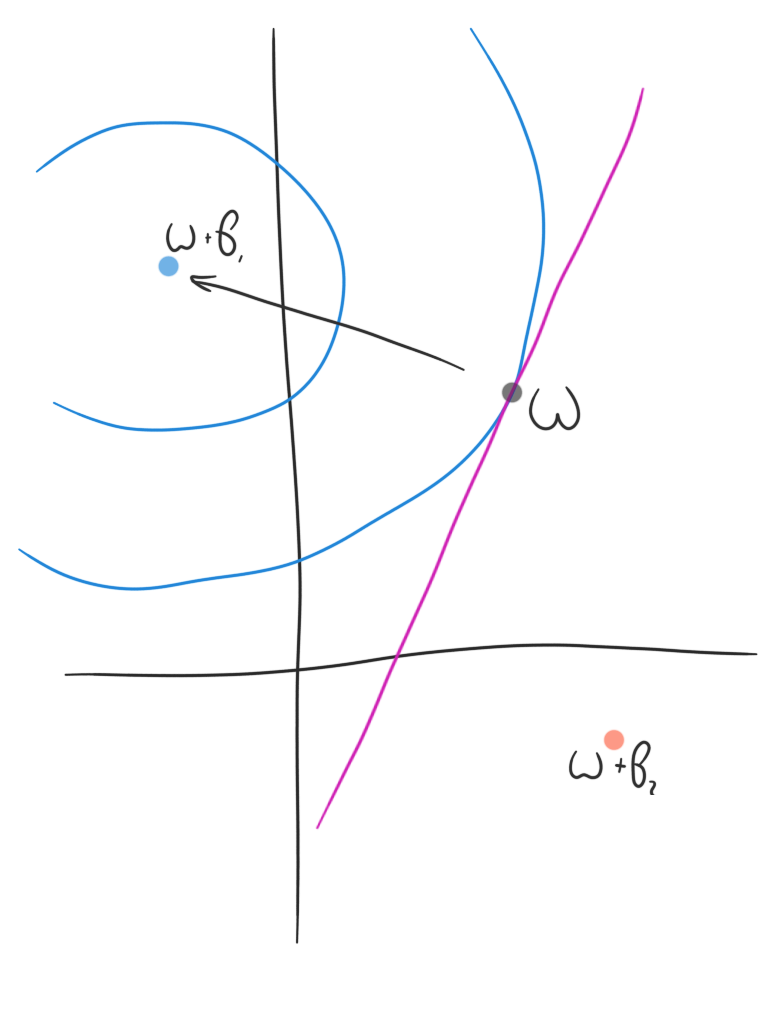
\includegraphics[scale=0.65]{pics/M4/battaglini02.png}
		\end{center}
	\end{column}
	\begin{column}{0.5\textwidth}
		{\small
			\begin{itemize}
				\item Ask player $i$ to project the state on some axis orthogonal to $b_i$ and report the result.
				\item Will report honestly (i.e., report, which is a projection of $\omega +b_1$, coincides with the projection of the actual $\omega$).
				\item So we learn one coordinate of the true state.
			\end{itemize}
		}
	\end{column}
\end{columns}
\end{frame}


\begin{frame}{Idea}
\begin{columns}
	\begin{column}{0.5\textwidth}
		\begin{center}
			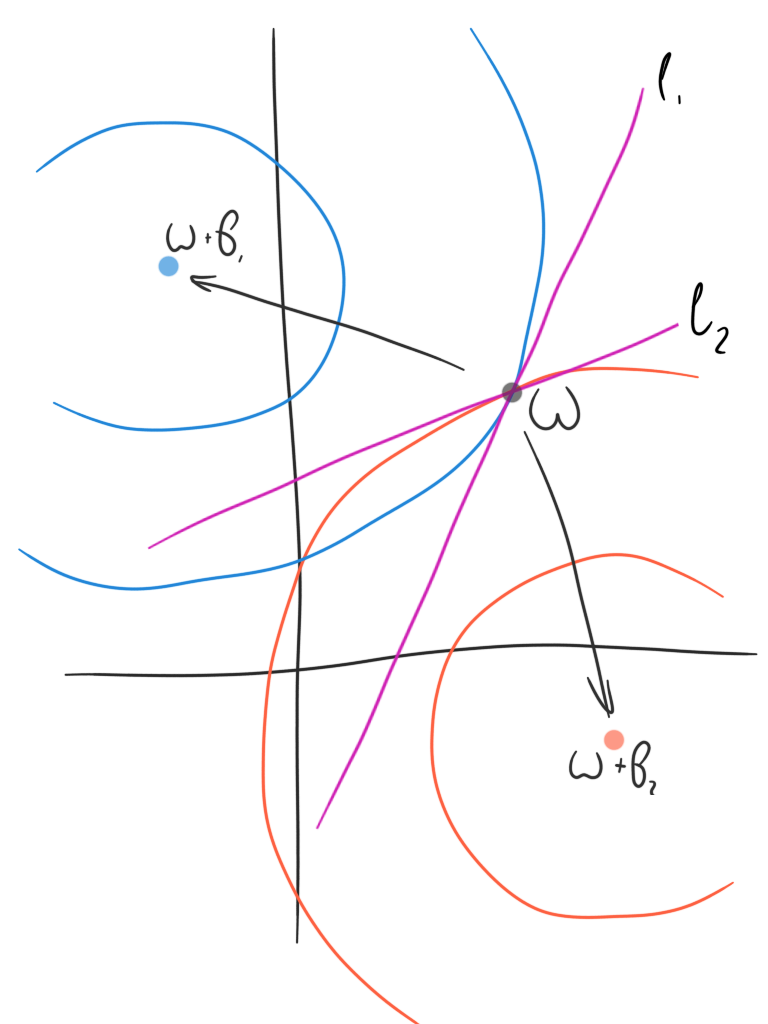
\includegraphics[scale=0.65]{pics/M4/battaglini03.png}
		\end{center}
	\end{column}
	\begin{column}{0.5\textwidth}
		{\small
			\begin{itemize}
				\item Then with two players, we can learn state perfectly this way.
				\item (As long as $b_i$ \structure{linearly independent}.)
				\item More generally, two players are enough to learn the state of any dimensionality $n$, since asking either player allows to learn $n-1$ dimensions of state.
				\item See Battaglini (2003) for $n$ dimensions and more general preferences.
			\end{itemize}
		}
	\end{column}
\end{columns}
\end{frame}


\begin{frame}{Equilibrium strategies}
\begin{columns}
	\begin{column}{0.5\textwidth}
		\begin{center}
			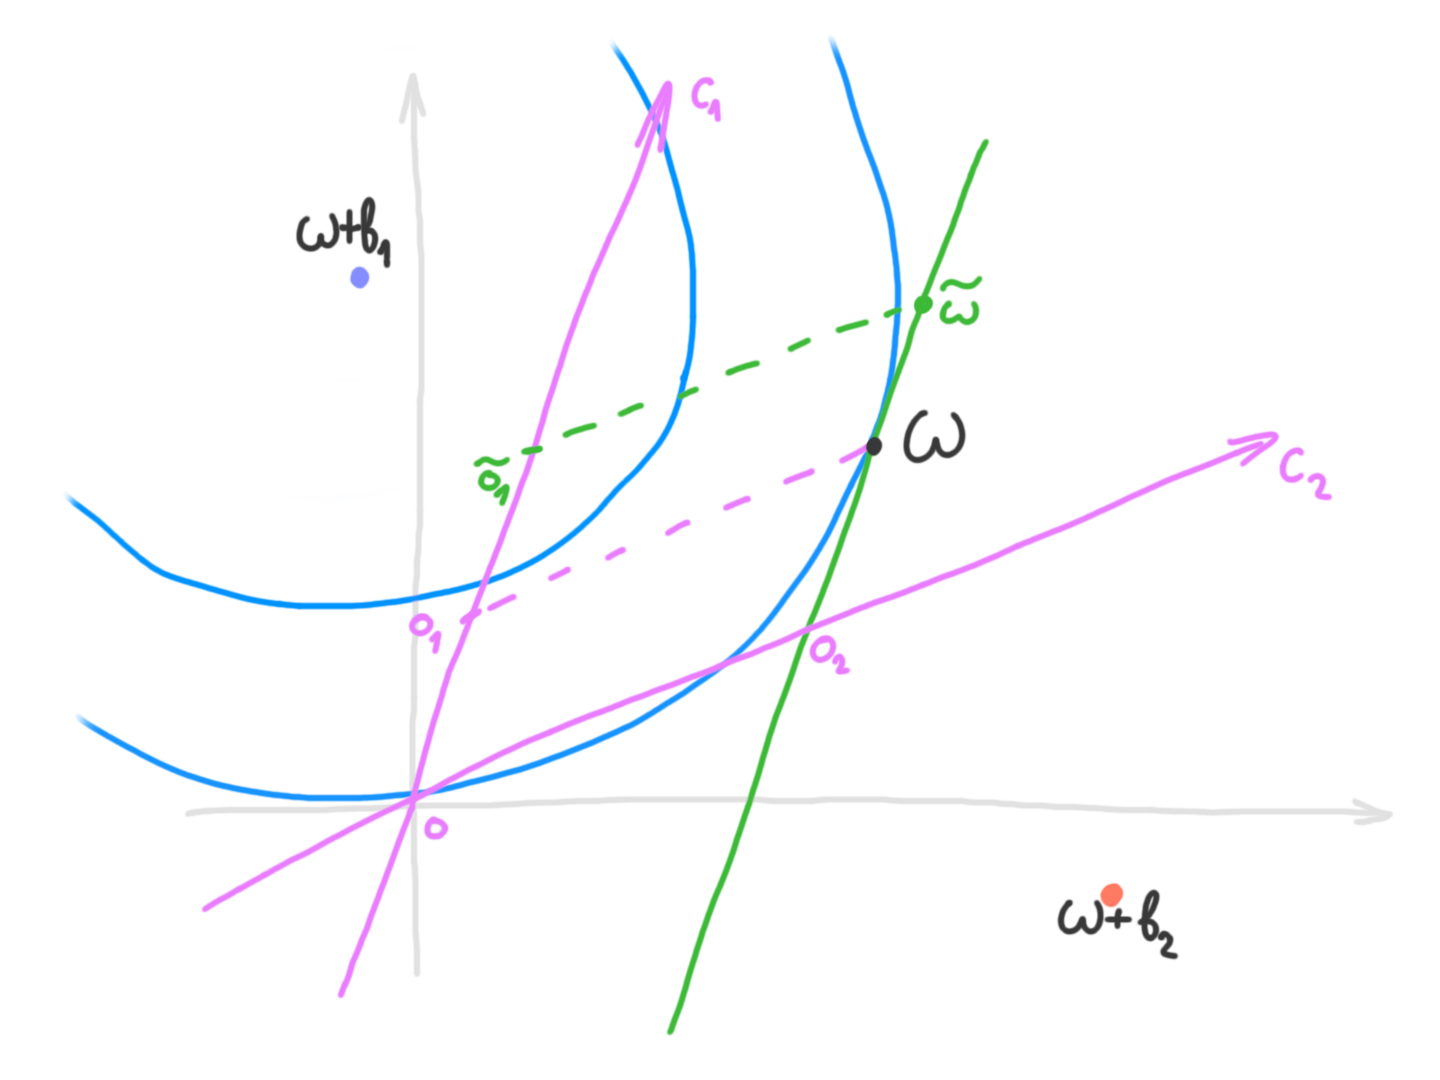
\includegraphics[scale=0.65]{pics/M4/battaglini04.png}
		\end{center}
	\end{column}
	\begin{column}{0.5\textwidth}
		{\small
			\begin{itemize}
				\item Consider basis $(c_1,c_2)$ where $b_i \perp c_i \in \mathbb{R}^2$ -- i.e., $b_i \cdot c_i = 0$ ($\iff b_i^1 c_i^1 + b_i^2 c_i^2 = 0$). 
				\item State $\omega$ has unique coordinates $(o_1,o_2)$ in this basis, i.e. $\omega = o_1 \cdot c_1 + o_2 \cdot c_2$.
				\item Ask A1 to report $o_1$. If A2 reports $o_2$ truthfully, A1 effectively chooses an action on the green line (see graph). 
				\item So truthful reporting is optimal for A1 (green line is orthog to $b_1$ $\Rightarrow$ it is tangent to A1's circular indifference curve at $\omega$ $\Rightarrow$ any lies $\tilde{o}_1$ puts the implemented action $\tilde{\omega}$ on a lower indiff curve).
			\end{itemize}
		}
	\end{column}
\end{columns}
\end{frame}


\begin{frame}{Clarifications}
	\begin{itemize}
		\item There are many vectors $c_i$ that are orthogonal to a given $b_i$ -- select any.
		\begin{itemize}
			\item E.g., letting $c_i = \frac{1}{\left\| b_i \right\|_2 } \left[ \begin{array}{c c} 0 & 1 \\ -1 & 0 \end{array} \right] \left( \begin{array}{c}
				b_i^1 \\ b_i^2
			\end{array} \right)$ would yield a vector $c_i$ of unit length that is rotated $90\deg$ clockwise w.r.t. $b_i$.
		\end{itemize}
		\item Formally, the problem setup says that messages are two-dimensional: $m_i \in \mathbb{R}^2$. So to be 100\% formal you can say that, e.g., $m_i = (o^i, 0)$, and that the principal ignores the second coordinate of each message.
		\begin{itemize}
			\item Alternatively: agents are expected to report $\omega$, but then the principal calculated respective $o_i$ and decides based on them (even (especially!) if reports do not coincide).
		\end{itemize}
	\end{itemize}
\end{frame}


\begin{frame}{Correlated information: Conclusion}
\begin{itemize}
	\item \structure{Correlated information} can be \alert{\textbf{very} easily exploited}; many ways to do so:
	\begin{itemize}
		\item If players' preferences conflict -- set them against each other (divide et impera);
		\item If players' preferences same -- force them to verify each other's reports.
	\end{itemize}
	\item Of course there are always issues that can arise:
	\begin{itemize}
		\item If players can communicate outside of the mechanism, collusion is a real threat.
		\item Cross-vefication may require making incredible or infeasible threats.
	\end{itemize}
\end{itemize}
\end{frame}


%TODO: mention a paper about robust corrinfo exploits


\end{document}